\section{Inclusive $\Vzeros$ Analysis: Comparison the PWG-LF Results}
\label{sec:c03InclusiveV0s}

The strategy of the inclusive $\Vzero$ analysis is described
in~\cite{Ali2012:ana501,Ali2013:ana702}.
In the following,
a short summary about the details of the inclusive $\Vzero$ analysis
as well as some general discussions will be given
in the first three parts of this section.
Then, the comparisons of the inclusive $\Vzero$ spectra between
LF analysis and this analysis will be presented.
At final, we will claim that,
the discrepancy between the results in LF analysis and this analysis
is mainly caused by the event selection criteria used in LF analysis and
JE framework are different.

\subsection{Event selection of inclusive $\Vzero$ analysis}
\label{sec:c03EventSel}

The event selection in the inclusive $\Vzero$
analysis~\cite{Ali2012:ana501,Ali2013:ana702}
is not exactly the same
as that in EMCal jet framework,
the differences are:
\begin{itemize}
\item this analysis is based on AOD (as shown in
      section~\ref{sec:02DataSample}) and LF analysis is based on ESD;
\item in this analysis,
      the event vertex is selected by using the pA 2013 vertex selection
      method in {\bf AliAnalysisUtils},
      this method requires the event should have the stable reconstructed
      vertex with TPC tracks,
      but this requirement is removed in the vertex selection criteria
      in LF analysis:
      \begin{lstlisting}
AliESDEvent *lESDevent = dynamic_cast<AliESDEvent*>(InputEvent());
const AliESDVertex *vertex = lESDevent->GetPrimaryVertexTracks();

Bool_t fHasVertex = kFALSE;
if (vertex->GetNContributors()<1) {
  vertex = lESDevent->GetPrimaryVertexSPD();
  if (vertex->GetNContributors()<1)
    fHasVertex = kFALSE;
  else
    fHasVertex = kTRUE;

  Double_t cov[6]={0};
  vertex->GetCovarianceMatrix(cov);
  Double_t zRes = TMath::Sqrt(cov[5]);

  TString vtxTyp = vertex->GetTitle();
  if (vtxTyp.Contains("vertexer:Z") && (zRes>0.25)) fHasVertex = kFALSE;
} else {
  fHasVertex = kTRUE;
}
      \end{lstlisting}
\item no pileup rejection in the LF analysis.
\end{itemize}

\begin{figure}[htbp]
\begin{center}
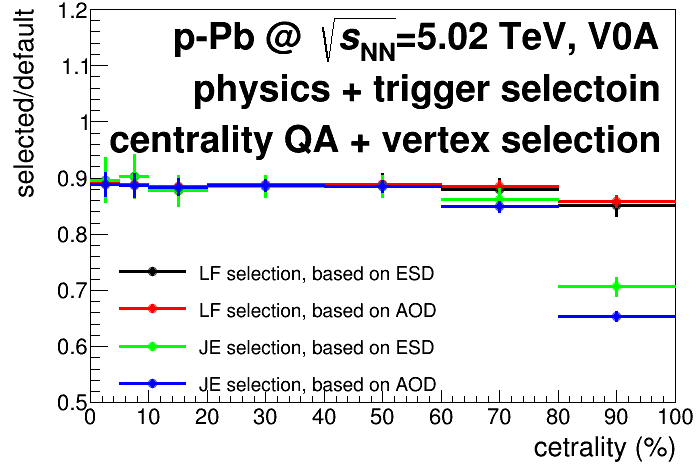
\includegraphics[width=.48\textwidth]{c03EvSel/ccomp_Sel_Vertex}
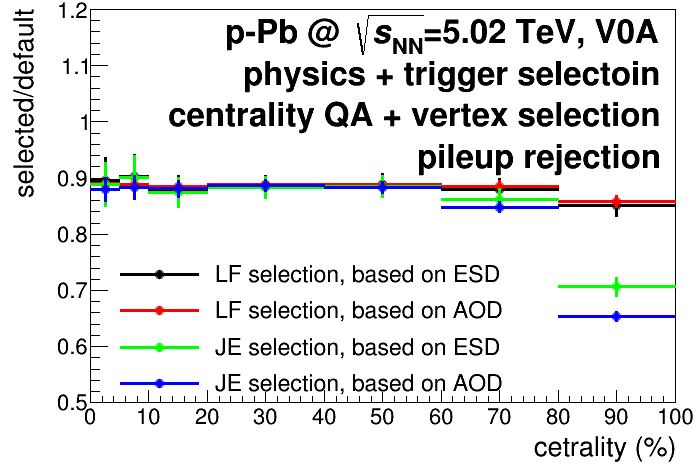
\includegraphics[width=.48\textwidth]{c03EvSel/ccomp_Sel_Pileup}
\caption{Comparison of the LF and JE event selection criteria,
         see the texts for the details.}
\label{fig:c03CompEventSel}
\end{center}
\end{figure}

Figure~\ref{fig:c03CompEventSel} shows the ratios between the number of events
with the given selection cuts in both AOD and ESD.
The "default" cuts are the event trigger selection and centrality QA.
These two cuts are the same in both LF analysis and this analysis.
In the left panel of figure~\ref{fig:c03CompEventSel},
the ratios are built between the results with the additional
vertex selections and the default one.
The pileup rejection is added in the ratios in the right panel of
figure~\ref{fig:c03CompEventSel}.
The comparisons show that,
the JE vertex selection rejects more events in the peripheral collisions than
the LF vertex selection.
And with a given vertex selection,
the different between AOD and ESD is small.
This difference can be caused by the definitions of the primary vertex in
AOD and that in ESD are different.
Anyhow, the effect of the pileup rejection is small in
LHC13b and LHC13c periods.
And it is not expected to change the final results dramatically.

\subsection{$\Vzero$ candidate selection}\label{sec:c03V0CandiSel}

In both data and MC, the online $\Vzeros$ are used in the analysis.

\begin{table}[htdp]
\begin{center}
\begin{tabular}{|c|c|}
\hline
selection                      & value \\
\hline
$\Vzero$ 2D decay radius       & in $[0.5,200]$~cm \\
negative track DCA to PV       & $>0.06$~cm \\
positive track DCA to PV       & $>0.06$~cm \\
DCA between $\Vzero$ daughters & $<1\sigma$ \\
$\cos\theta_{\rm pointing}$    & $>0.97$ ($\Kshort$), $>0.995$ ($\Lambda$) \\
\hline
\end{tabular}
\end{center}
\caption{Default cuts for $\Vzero$ decay topological selection.}
\label{tab:c03ValSelV0Topo}
\end{table}

\begin{table}[htdp]
\begin{center}
\begin{tabular}{|c|c|}
\hline
selection                           & value \\
\hline
track Kink index                    & $<1$ \\
$|\eta|$                            & $<0.8$ \\
TPC refit flag                      & kTRUE \\
number of crossed rows in TPC       & $>70$ \\
number of findable rows in TPC      & $>0$ \\
crossed rows / findable rows ratio  & $>0.8$ \\
TPC ${\rm d}E/{\rm d}x$             & $<5\sigma$ \\
\hline
\end{tabular}
\end{center}
\caption{Default selection cuts for $\Vzero$ daughter tracks.}
\label{tab:c03ValSelV0DauTrk}
\end{table}

In data, the $\Vzero$ candidates are selected by several set of cuts:
\begin{itemize}
\item $\Vzero$ secondary vertex reconstruction with $\chi^{2}<33$;
\item topological selection;
\item daughter track selection;
\item proper lifetime ($mL/p$):
      default value for $\Kshort$ ($\Lambda$) is $<20$~cm ($<30$~cm);
\item invriant mass restriction (as a function of $\Vzero$ $\pT$):
      \begin{itemize}
      \item $\Kshort$:
            \begin{itemize}
            \item upper band: $0.563707+0.0114979\times\pT$,
            \item lower band: $0.430006-0.0110029\times\pT$,
            \end{itemize}
      \item $\Lambda$ and $\AntiLa$:
            \begin{itemize}
            \item upper band:
                  $1.13688+0.00527838\pT+0.084222\times\exp(-3.80595\pT)$,
            \item lower band:
                  $1.09501-0.00523272\pT-0.075269\times\exp(-3.46339\pT)$;
            \end{itemize}
      \end{itemize}
\item competing $\Vzero$ rejection:
      \begin{itemize}
      \item $\Kshort$: $|M_{{\rm p}\pim}-M_{\Lambda}|>0.005~\GeVcc$ and 
                       $|M_{\pbar\pip}-M_{\AntiLa}|>0.005~\GeVcc$,
      \item $\Lambda$ and $\AntiLa$: $|M_{\pip\pim}-M_{\Kshort}|>0.01~\GeVcc$.
      \end{itemize}
\end{itemize}
The default cut values for the $\Vzero$ decay topology and $\Vzero$
daughter tracks are listed in table~\ref{tab:c03ValSelV0Topo}
and~\ref{tab:c03ValSelV0DauTrk}.

In MC, the reconstructed $\Vzeros$ and the decay daughter tracks are
identified by the MC truth information.
To build the numerator of the efficiency,
the $\Vzeros$ candidates are selected by using the exactly the cuts as
in data except the daughter track PID with ${\rm d}E/{\rm d}x$ in TPC.

\subsection{Analysis strategy}\label{sec:c03AnaStrategy}

\begin{figure}[htb]
\begin{center}
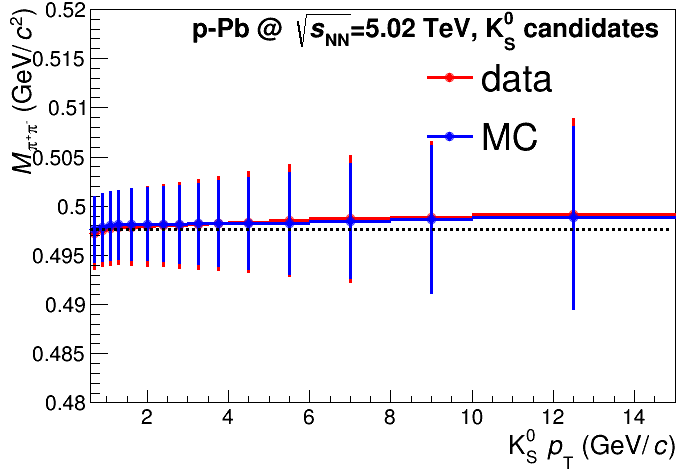
\includegraphics[width=.32\textwidth]{c03SigExtra/ccompKshortFitInvM}
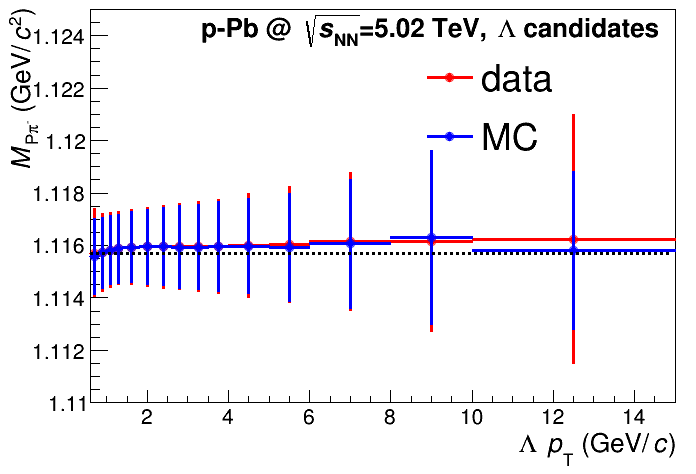
\includegraphics[width=.32\textwidth]{c03SigExtra/ccompLambdaFitInvM}
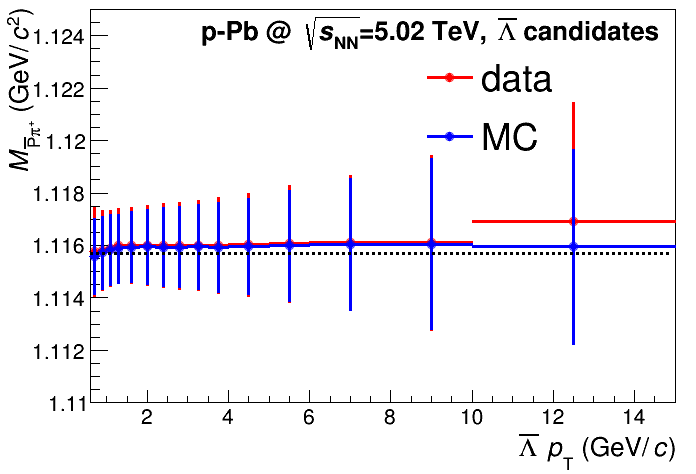
\includegraphics[width=.32\textwidth]{c03SigExtra/ccompAntiLaFitInvM}
\caption{The centre value and width of the $\Vzero$ candidates invariant mass
         distribution from the Gaussian fit.
         The results are shown as a function of $\pT$ and they are obtained
         in $0-5\%$ event multiplicity bin with the V0A estimator.}
\label{fig:c03FitInvM}
\end{center}
\end{figure}

The strategy of the inclusive $\Vzero$ analysis includes the following steps:
\begin{itemize}
\item Extract raw spectra in data:
      \begin{enumerate}
      \item fit $\Vzero$ invariant mass distribution with Gaussian plus a
            linear function in each $\pT$ bin and extract the
            mean ($M_{\rm mean}$) and $\sigma$ of the Gaussian;
      \item define the $\Vzero$ signal window as
            $M_{\rm mean}\pm N\sigma$ (the default option is $N=6$);
      \item fit the combinatorial background in the side
            bands ($[-2N\sigma+M_{\rm mean},-N\sigma+M_{\rm mean}]$
            and $[N\sigma+M_{\rm mean},2N\sigma+M_{\rm mean}]$)
            and interpolate it into the signal window;
      \item subtract the interpolated background from the counts in
            signal window and extract the raw yield of $\Vzeros$ in
            each $\pT$ bin.
      \end{enumerate}
\item Build correction efficiency in MC:
      \begin{enumerate}
      \item reproduce step $3$ and $4$ with the $M_{\rm mean}$ and $\sigma$
            extracted in data for the physical primary $\Vzeros$ at detector
            level in MC to define the numerator of the efficiency;
      \item the denominator of the efficiency is built by the physical primary
            particles at generation level;
      \item for $\Lambda$ and $\AntiLa$, the $\Xi$ feeddown component,
            which is evaluated by scaling the yield of feeddown $\Lambda$
            and $\AntiLa$ in MC according to the measured $\Xi$ spectra in data,
            have to be subtracted before the efficiency correction (details
            are described in~\cite{Ali2012:ana501}).
      \end{enumerate}
\end{itemize}

Figure~\ref{fig:c03FitInvM} shows the centre value and width (the error bar)
of the $\Vzero$ candidates invariant mass distribution from the Gaussian
fit~\footnote{In data,
the signal peak is fitted by the Gaussian plus a linear function and in MC
the signal peak is fitted by the Gaussian alone.}
in $0-5\%$ event multiplicity bin with the V0A estimator.
The results are shown as a function of $\pT$.
There is very good agreement for the centre points between the data and MC.
In general, the width of the invariant mass distribution in MC is smaller
than that in data.
This is due to the invariant mass distribution of $\Vzero$ candidates in MC
is built by the MC truth $\Vzero$ and there is no combinatorial background.
The parameters obtained in data (the red curves) are used to build the
$\pT$-dependent signal window and side bands for the background subtraction
in both data and MC.

\begin{figure}[htb]
\begin{center}
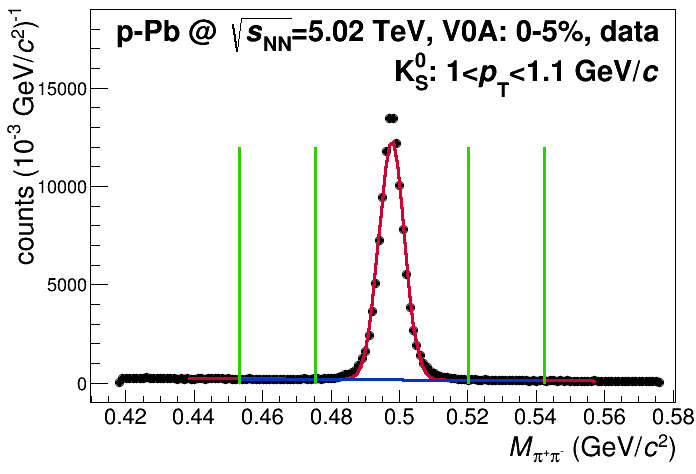
\includegraphics[width=.49\textwidth]{c03SigExtra/cPlotFitInvM_RD}
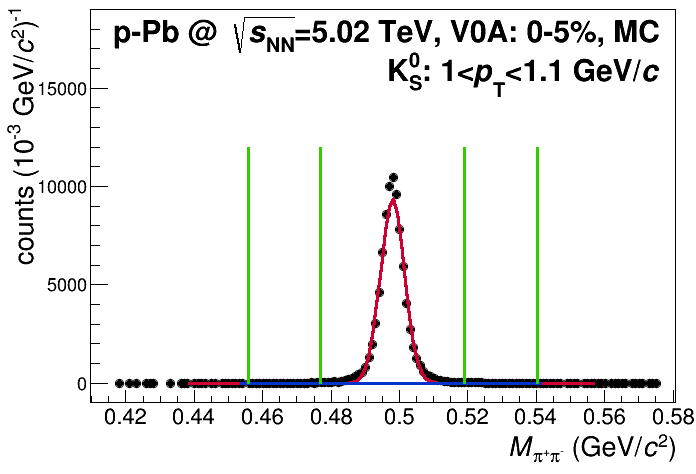
\includegraphics[width=.49\textwidth]{c03SigExtra/cPlotFitInvM_MC}
\caption{Bin counting fits of the $\Vzero$ invariant mass distributions in data (left) and in MC (right).
The $\Kshort$ candidates in $1<\pT<1.1~\GeVc$ and the most central collisions ($0-5\%$) are
chosen as an example.}
\label{fig:c03FitCbinV0s}
\end{center}
\end{figure}

As mentioned in section~\ref{sec:c03V0CandiSel},
the numerator of the efficiency is built by the MC truth $\Vzeros$
and indeed, it does not contain the combinatory background.
To reproduce the procedure of the combinatory background subtraction
in MC is used to minimize the discrepancy between the data and MC.
Figure~\ref{fig:c03FitCbinV0s} shows the bin counting fits of the $\Kshort$
invariant mass distributions in data (left) and in MC (right) as an example.
In each of the plot:
\begin{itemize}
\item the red line shows the Gaussian fit of the signal peak;
\item the blue line is the built by interpolating the fit in the side bands
      into the signal window;
\item the signal window and the side bands,
      which are defined by $6\sigma$,
      are separated by the green lines~\footnote{As also shown in
      figure~\ref{fig:c03FitInvM}, the width of the $\Vzero$ invariant mass
      distriubiton in MC in smaller than that in data.
      Only the centre points and width extracted in data are used to
      calculate the efficiency.}.
\end{itemize}
One can notice that,
the counts in the side bands in MC is non-vanished even all the $\Vzeros$ are
identified by the MC truth information.
They are contributed by the $\Vzeros$ which have large daughter track $\pT$
resolution.
And the interpolation of the bin counting fit in the side bands (the blue line)
will also give a non-zero contribution in the signal region in the MC.
In this case, the interpolated bin counting fit in data not only contains the
combinatorial background but also includes the contribution of the
real $\Vzeros$ which located in the side bands.
Applying the background subtraction in data,
it will subtract both the combinatorial background and a fraction of
real $\Vzeros$.
To minimize this effect, the interpolated curve from the bin counting fit
in the side bands was also subtracted in signal window in MC in the
efficiency calculation.

\begin{figure}[htb]
\begin{center}
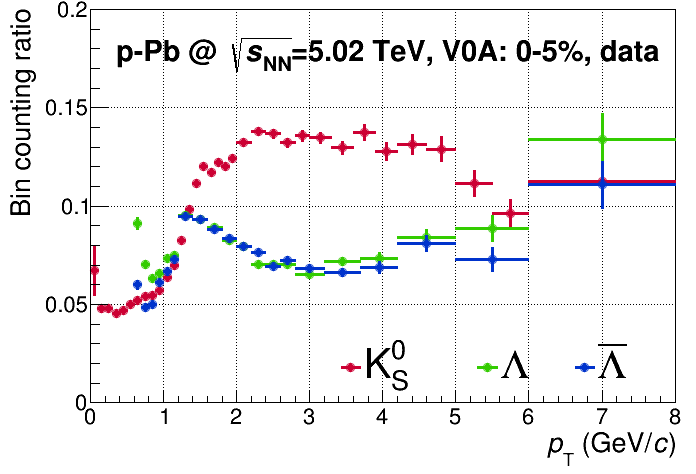
\includegraphics[width=.49\textwidth]{c03SigExtra/cCbinRatio_RD}
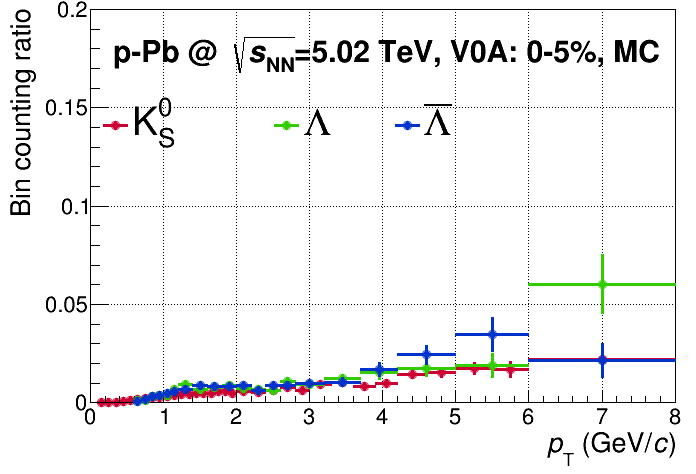
\includegraphics[width=.49\textwidth]{c03SigExtra/cCbinRatio_MC}
\caption{The bin counting ratio for $\Vzeros$ as a function of $\pT$ in data (left) and in MC (right).
The results are obtained in $0-5\%$ event multiplicity bin with V0A estimator.
More details are in the texts.}
\label{fig:c03CbinRatio}
\end{center}
\end{figure}

Figure~\ref{fig:c03CbinRatio} shows the ratio between the interpolated curve
in the signal window (the blue lines in figure~\ref{fig:c03FitCbinV0s}) and
the counts in the signal window after subtracting the interpolated curve in
data (left) and in MC (right):
\begin{equation}\label{eq:c03CbinR}
R_{\rm Cbin}=\frac{N_{\rm interp}}{N_{\rm SW}-N_{\rm interp}},
\end{equation}
where, $N_{\rm interp}$ is the value of the interpolated curve and
$N_{\rm SW}$ is the counts in the signal window.
Here, we define it as the "bin counting ratio" ($R_{\rm Cbin}$).
Indeed, this ratio is defined as the background-to-signal ratio of the
inclusive $\Vzeros$ in data in~\cite{Ali2012:ana501}.
In MC, this ratio has the non-vanish value and it is around $1\%$ in low and
intermediate $\pT$ regions (the right panel of figure~\ref{fig:c03CbinRatio}),
but large fluctuations are found at high $\pT$.
These fluctuations will be included in the systematic uncertainty of the
final results (see the discussion in section~\ref{sec:c06SystSingleV0s}).

\subsection{Comparison to the LF results}

In this analysis,
to measure the production of $\Vzeros$ in jets,
we derived the analysis task based on the EMCal jet framework,
which fills the jets and $\Vzeros$ into two independent tree branches,
and the events are selected according the criteria in EMcal jet framework.
As the first step of this analysis, to validate our analysis code,
we compared the $\Vzeros$ spectra in our measurement to those of the LF.
As discussed in section~\ref{sec:c03EventSel},
the event selection criteria in LF analysis and those in EMCal jet framework
are not the same and their effects are different,
especially in the peripheral collisions (see figure~\ref{fig:c03CompEventSel}).
To ensure the comparison is done under the same conditions,
we modified the EMcal jet framework (privately) and used the same event
and $\Vzero$ selection criteria as those in LF analysis.
Our measurement is based on one run (run 195568,
$\sim 1.2\time 10^{7}$ events) in ESD.
The LF resutls are from~\cite{Abelev:2013haa}.
The $\Vzeros$ are selected in $0<y_{\rm CMS}<0.5$.

\begin{figure}[htb]
\begin{center}
\includegraphics[width=.32\textwidth]{c03ESD/cKshort_CompLF_V0A_000_005}
\includegraphics[width=.32\textwidth]{c03ESD/cLambda_CompLF_V0A_000_005}
\includegraphics[width=.32\textwidth]{c03ESD/cAntiLa_CompLF_V0A_000_005}
\caption{Compare to LF results, $0-5\%$.}
\label{fig:c03Comp000005ESD}
\end{center}
\end{figure}

\begin{figure}[htb]
\begin{center}
\includegraphics[width=.32\textwidth]{c03ESD/cKshort_CompLF_V0A_005_010}
\includegraphics[width=.32\textwidth]{c03ESD/cLambda_CompLF_V0A_005_010}
\includegraphics[width=.32\textwidth]{c03ESD/cAntiLa_CompLF_V0A_005_010}
\caption{Compare to LF results, $5-10\%$.}
\label{fig:c03Comp005010ESD}
\end{center}
\end{figure}

\begin{figure}[htb]
\begin{center}
\includegraphics[width=.32\textwidth]{c03ESD/cKshort_CompLF_V0A_010_020}
\includegraphics[width=.32\textwidth]{c03ESD/cLambda_CompLF_V0A_010_020}
\includegraphics[width=.32\textwidth]{c03ESD/cAntiLa_CompLF_V0A_010_020}
\caption{Compare to LF results, $10-20\%$.}
\label{fig:c03Comp010020ESD}
\end{center}
\end{figure}

\begin{figure}[htb]
\begin{center}
\includegraphics[width=.32\textwidth]{c03ESD/cKshort_CompLF_V0A_020_040}
\includegraphics[width=.32\textwidth]{c03ESD/cLambda_CompLF_V0A_020_040}
\includegraphics[width=.32\textwidth]{c03ESD/cAntiLa_CompLF_V0A_020_040}
\caption{Compare to LF results, $20-40\%$.}
\label{fig:c03Comp020040ESD}
\end{center}
\end{figure}

\begin{figure}[htb]
\begin{center}
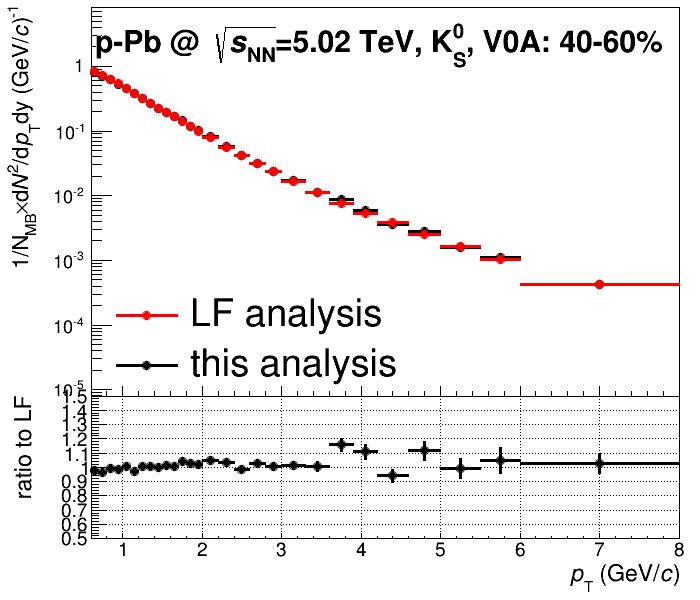
\includegraphics[width=.32\textwidth]{c03ESD/cKshort_CompLF_V0A_040_060}
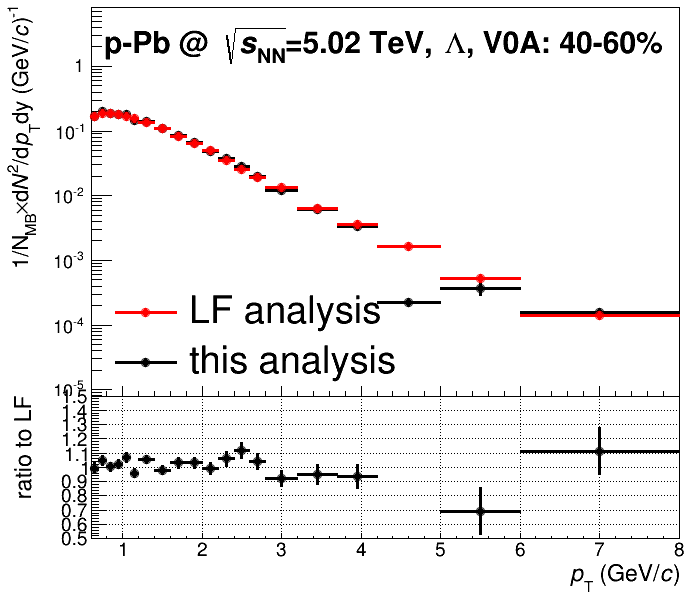
\includegraphics[width=.32\textwidth]{c03ESD/cLambda_CompLF_V0A_040_060}
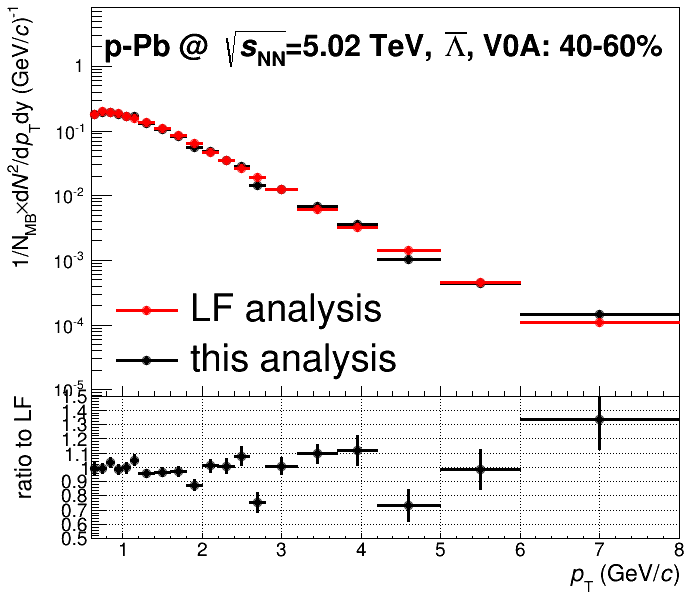
\includegraphics[width=.32\textwidth]{c03ESD/cAntiLa_CompLF_V0A_040_060}
\caption{Compare to LF results, $40-60\%$.}
\label{fig:c03Comp040060ESD}
\end{center}
\end{figure}

\begin{figure}[htb]
\begin{center}
\includegraphics[width=.32\textwidth]{c03ESD/cKshort_CompLF_V0A_060_080}
\includegraphics[width=.32\textwidth]{c03ESD/cLambda_CompLF_V0A_060_080}
\includegraphics[width=.32\textwidth]{c03ESD/cAntiLa_CompLF_V0A_060_080}
\caption{Compare to LF results, $60-80\%$.}
\label{fig:c03Comp060080ESD}
\end{center}
\end{figure}

\begin{figure}[htb]
\begin{center}
\includegraphics[width=.32\textwidth]{c03ESD/cKshort_CompLF_V0A_080_100}
\includegraphics[width=.32\textwidth]{c03ESD/cLambda_CompLF_V0A_080_100}
\includegraphics[width=.32\textwidth]{c03ESD/cAntiLa_CompLF_V0A_080_100}
\caption{Compare to LF results, $80-100\%$.}
\label{fig:c03Comp080100ESD}
\end{center}
\end{figure}

The comparisons are presented in seven event multiplicity bins,
the results are shown
in figure~\ref{fig:c03Comp000005ESD}~to figure~\ref{fig:c03Comp080100ESD}.
These two analyses are consistent within the statistic errors in all
event multiplicity bins.

\begin{figure}[htb]
\begin{center}
\includegraphics[width=.32\textwidth]{c03AOD/cKshort_CompLF_V0A_000_005}
\includegraphics[width=.32\textwidth]{c03AOD/cLambda_CompLF_V0A_000_005}
\includegraphics[width=.32\textwidth]{c03AOD/cAntiLa_CompLF_V0A_000_005}
\caption{Compare to LF results, $0-5\%$.
         $\Vzero$ sepectra in this analysis is obtained with the
         JE event selection criteria.}
\label{fig:c03Comp000005AOD}
\end{center}
\end{figure}

\begin{figure}[htb]
\begin{center}
\includegraphics[width=.32\textwidth]{c03AOD/cKshort_CompLF_V0A_005_010}
\includegraphics[width=.32\textwidth]{c03AOD/cLambda_CompLF_V0A_005_010}
\includegraphics[width=.32\textwidth]{c03AOD/cAntiLa_CompLF_V0A_005_010}
\caption{Compare to LF results, $5-10\%$.
         $\Vzero$ sepectra in this analysis is obtained with the
         JE event selection criteria.}
\label{fig:c03Comp005010AOD}
\end{center}
\end{figure}

\begin{figure}[htb]
\begin{center}
\includegraphics[width=.32\textwidth]{c03AOD/cKshort_CompLF_V0A_010_020}
\includegraphics[width=.32\textwidth]{c03AOD/cLambda_CompLF_V0A_010_020}
\includegraphics[width=.32\textwidth]{c03AOD/cAntiLa_CompLF_V0A_010_020}
\caption{Compare to LF results, $10-20\%$.
         $\Vzero$ spectra in this analysis is obtained with the
         JE event selection criteria.}
\label{fig:c03Comp010020AOD}
\end{center}
\end{figure}

\begin{figure}[htb]
\begin{center}
\includegraphics[width=.32\textwidth]{c03AOD/cKshort_CompLF_V0A_020_040}
\includegraphics[width=.32\textwidth]{c03AOD/cLambda_CompLF_V0A_020_040}
\includegraphics[width=.32\textwidth]{c03AOD/cAntiLa_CompLF_V0A_020_040}
\caption{Compare to LF results, $20-40\%$.
         $\Vzero$ spectra in this analysis is obtained with the
         JE event selection criteria.}
\label{fig:c03Comp020040AOD}
\end{center}
\end{figure}

\begin{figure}[htb]
\begin{center}
\includegraphics[width=.32\textwidth]{c03AOD/cKshort_CompLF_V0A_060_080}
\includegraphics[width=.32\textwidth]{c03AOD/cLambda_CompLF_V0A_060_080}
\includegraphics[width=.32\textwidth]{c03AOD/cAntiLa_CompLF_V0A_060_080}
\caption{Compare to LF results, $60-80\%$.
         $\Vzero$ spectra in this analysis is obtained with the
         JE event selection criteria.}
\label{fig:c03Comp060080AOD}
\end{center}
\end{figure}

\begin{figure}[htb]
\begin{center}
\includegraphics[width=.32\textwidth]{c03AOD/cKshort_CompLF_V0A_080_100}
\includegraphics[width=.32\textwidth]{c03AOD/cLambda_CompLF_V0A_080_100}
\includegraphics[width=.32\textwidth]{c03AOD/cAntiLa_CompLF_V0A_080_100}
\caption{Compare to LF results, $80-100\%$.
         $\Vzero$ spectra in this analysis is obtained with the
         JE event selection criteria.}
\label{fig:c03Comp080100AOD}
\end{center}
\end{figure}

Figure~\ref{fig:c03Comp000005AOD} to figure~\ref{fig:c03Comp080100AOD}
are the comparisons of the results in LF and JE analyses.
The same as figure~\ref{fig:c03Comp000005ESD} to
figure~\ref{fig:c03Comp080100ESD},
the LF results come from ref.~\cite{Abelev:2013haa}.
But the results in this analysis is obtained with the JE event and selections
and based on AOD.
The two analyses are consistent in the central and semi-central collisions,
but the deviation is found in the peripheral collisions.

\begin{figure}[!htb]
\begin{center}
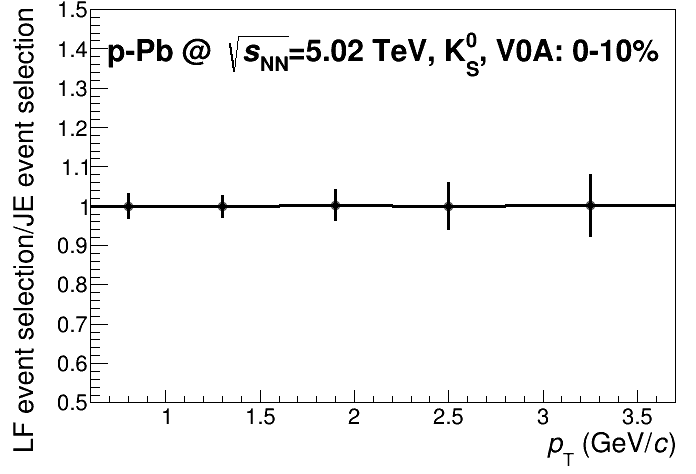
\includegraphics[width=.48\textwidth]{c03EvSel/ccomp_Ka_Ratio_V0A_000_010}
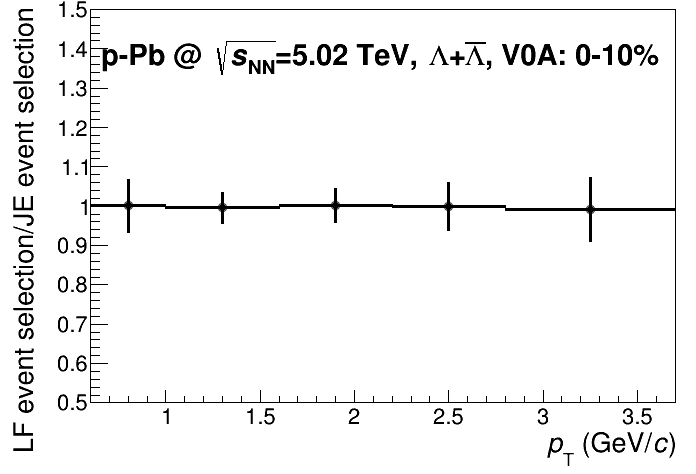
\includegraphics[width=.48\textwidth]{c03EvSel/ccomp_La_Ratio_V0A_000_010}
\caption{Comparison of the $\Vzero$ candidate multiplicities
         in LF and JE analysis in central collisions,
         details are in the texts.}
\label{fig:c03CompMultiV0s000010}
\end{center}
\end{figure}

\begin{figure}[!htb]
\begin{center}
\includegraphics[width=.48\textwidth]{c03EvSel/ccomp_Ka_Ratio_V0A_080_100}
\includegraphics[width=.48\textwidth]{c03EvSel/ccomp_La_Ratio_V0A_080_100}
\caption{Comparison of the $\Vzero$ candidate multiplicities
         in LF and JE analysis in central collisions,
         details are in the texts.}
\label{fig:c03CompMultiV0s080100}
\end{center}
\end{figure}

This deviation in the peripheral collisions can be explained by the
comparisons shown in figure~\ref{fig:c03CompEventSel}.
For more details,
we compared the ratio of the per-event multiplicity of $\Vzero$ candidates
as a function of $\pT$ with JE and LF event selections, respectively.
The comparisons are shown in figure~\ref{fig:c03CompMultiV0s000010} (for
central collisions) and in figure~\ref{fig:c03CompMultiV0s080100} (for
peripheral collisions) with the V0A event multiplicity estimator.
The $\Vzero$ candidates are selected by the cuts defined in
section~\ref{sec:c03V0CandiSel},
the cut on the invariant mass is also applied
but without the combinatory background subtraction.
In the central collisions ($0-10\%$, figure~\ref{fig:c03CompMultiV0s000010}),
the JE analysis LF analysis give the exactly the same results which is
consistent with the conclusion in figutre~\ref{fig:c03CompEventSel}.
But in the peripheral collisions,
the $\Vzero$ mutliplicity in JE analysis is higher than that in the LF analysis.
The tighter vertex selection criteria implemented in the EMcal jet framework
rejects the lower multiplicity events w.~r.~t. the LF analysis and makes
the $\Vzero$ spectra in this analysis is systematically higher than those in
the LF analysis~\footnote{We have discussed the discrepancy in the peripheral
collisions between these two analysis with the LF people.
And they claimed that, this discrepancy could be caused by the cut of
the $\cos\theta_{\rm pointing}$ (see section~\ref{sec:c03V0CandiSel}).
Due to when they first compared their $\Kshort$ results to the charged Kaons,
they found the very similar deviation in the peripheral collisions.
According to this,
they suggested to use the $\pT$-dependent $\cos\theta_{\rm pointing}$ cut
to decrease the discrepancy.
But if the discrepancy between our analysis and LF analysis is mainly caused
by the effect of the $\cos\theta_{\rm pointing}$ cut,
it has to be also found in the ESD based analysis,
and this is not the case.}.

\begin{figure}[htb]
\begin{center}
\includegraphics[width=.49\textwidth]{c03AOD/cRatioV_CompLF_V0A_000_005}
\includegraphics[width=.49\textwidth]{c03AOD/cRatioV_CompLF_V0A_005_010}
\includegraphics[width=.49\textwidth]{c03AOD/cRatioV_CompLF_V0A_040_060}
\includegraphics[width=.49\textwidth]{c03AOD/cRatioV_CompLF_V0A_080_100}
\caption{The comparison for the ratio of $(\Lambda+\AntiLa)/2\Kshort$
         in LF analysis and this analysis in $7$ event multliplicity bins.
         The input spectra are from figure~\ref{fig:c03Comp000005AOD} to
         figure~\ref{fig:c03Comp080100AOD}.}
\label{fig:c03CompRatioV0AOD}
\end{center}
\end{figure}

Indeed, the final results in this analysis is focused on
the $\Lambda$-to-$\Kshort$ ratio in jets.
It is interesting to see how the effects of the event selections on
the this ratio of the inclusive $\Vzeros$.
The ratio of $(\Lambda+\AntiLa)/2\Kshort$ in four event multiplicity bins
with the input spectra come from figure~\ref{fig:c03Comp000005AOD} to
figure~\ref{fig:c03Comp080100AOD} are compared
in figure~\ref{fig:c03CompRatioV0AOD}.
The error bar in the LF results corresponds the quadratically combined
statistic and systematic uncertainties.
Despite the difference in the spectra,
the ratios of $(\Lambda+\AntiLa)/2\Kshort$ in this analysis are consistent
with those in LF analysis within errors from the central to the peripheral
collisions.
The small bin-by-bin discrepancy between this two analyses is caused by
the bin counting fitting~\cite{Ali2012:ana501} to extract the number of
signals and to build the efficiency in the fine bins of $\pT$.
This procedure is sensitive to the analysis details.
